\section{Ringe (3)}
\subsection{Def. Ring (3.1)}
\label{Def. Ring}
\subsubsection{Ring}
\label{Ring}
En ring er en abelsk \nameref{Gruppe} $(R,+)$ med en yderligere
\nameref{Komposition} $\cdot: R \times R \rightarrow R$ kaldet
\textbf{multiplikation}. Denne skal tilfredsstille følgende 3 egenskaber:

\begin{enumerate}[(i)]
  \item Multiplikationen skal være \textbf{associativ}:
  \begin{equation*}
  (x \cdot y) \cdot z = x \cdot (y \cdot z)
  \end{equation*}
  for alle $x,y,z \in R$
  
  \item Der skal eksistere et \textbf{neutralt} element $1 \in R$, sådan at:
  \begin{equation*}
  1 \cdot x = x \quad \text{og}\quad x \cdot 1 = x
  \end{equation*}
  for alle $x \in R$
  
  \item Multiplikationen skal være \textbf{distributiv}:
  \begin{equation*}
  x \cdot(y + z) = x \cdot y + x \cdot z \quad \text{og}\quad (y + z) \cdot x =
  y \cdot x + z \cdot x
  \end{equation*}
  for alle $x,y,z \in R$
\end{enumerate}
Bemærk at 0 er det neutrale element i $(R, +)$.

\subsubsection{Delring}
\label{Delring}
En delmængde $S \subseteq R$ af en \nameref{Ring} R, kaldes en \textbf{delring}
hvis
\begin{enumerate}[(i)]
  \item $S$ er en \nameref{Undergruppe} af $(R, +)$
  \item $1 \in S$
  \item $xy \in S$ hvis $x, y \in S$
\end{enumerate}

\subsubsection{Nuldivisor}
\label{Nuldivisor}
Et element $x \in R \setminus \myset{0}$ kaldes en \textbf{nuldivisor}, hvis der
eksisterer et $y \in R \setminus \myset{0}$ sådan at $xy = 0$ eller $yx = 0$.

\textit{En nuldivisor er et ikke-nul element der under multiplikation med et
andet element afbilder til 0, altså det neutrale element for
gruppe-kompositionen, ikke ring-kompositionen. Disse findes ikke for $\Z$, men
findes f.eks. for $2\times2$ matricer.}

\subsubsection{Enhed}
\label{Enhed}
Et element $x \in R$ kaldes en \textbf{enhed}, hvis der eksisterer $y \in R$
sådan at $xy = yx = 1$. I dette tilfælde skriver vi $y$ som $x^{-1}$, altså den
inverse til $x$. Mængden af enheder i $R$ skrives $R^*$.

\textit{En enhed er et element der har en invers i forhold til multiplikation.}

\subsubsection{Def. 3.1.1}
\label{Def. 3.1.1}
Her følger nogle af de vigtigeste definitioner omkring ringe:
\begin{enumerate}[(i)]
  \item \nameref{Delring}.
  \item \nameref{Nuldivisor}.
  \item \nameref{Enhed}.
  \item Vi siger $R$ er \textbf{kommutativ} hvis $xy = yx$ for alle $x, y \in
  R$.
\end{enumerate}

Multiplikationen i $R$ gør $R^*$ til en \nameref{Gruppe}, $(R^*, \cdot)$. Hvis
$R \neq \myset{0}$, så $0 \nin R^*$. Gruppen af enheder i en kommutativ
\nameref{Ring} $R$ er en abelsk gruppe.

\subsubsection{Legeme}
\label{Legeme}
En \nameref{Ring} $R$ med $R^* = R\setminus \myset{0}$ kaldes et
\textbf{legeme}.

\textit{En ring er et legeme hvis alle elementer, foruden 0, har en invers i
forhold til multiplikation (alle elementer skal være \nameref{Enhed}er).}

\subsubsection{Integritetsområde}
\label{Integritetsomraade}
En \nameref{Ring}, $R \neq \myset{0}$, der ikke indeholder
\nameref{Nuldivisor}er ($xy = 0, x, y \neq 0$) kaldes et
\textbf{integritetsområde}.

\subsubsection{Del - og udvidelseslegeme}
\label{Del - og udvidelseslegeme}
Hvis $K \subseteq L$ er \nameref{Legeme}r og $K$ er en \nameref{Delring} af $L$
så er $K$ et \textbf{dellegeme} af $L$, og $L$ er et \textbf{udvidelseslegeme} af $K$.


\subsubsection{Prop. 3.1.3}
\label{Prop. 3.1.3}
Lad $R$ være et \nameref{Integritetsomraade} og $a, x, y \in R$. Hvis $a \neq 0$
og $ax = ay$ så er $x = y$.

\subsubsection{Prop. 3.1.4}
\label{Prop. 3.1.4}
Lad $\F$ være et \nameref{Legeme}. Så er $\F$ et \nameref{Integritetsomraade}.

\textit{Et legeme indeholder ingen \nameref{Nuldivisor}er.}

\subsubsection{Talmængerne $\Z$, $\Q$, $\R$ og $\C$}
\label{Talmaengerne_Z_Q_R og C}
$\Z$ er en \nameref{Delring} af $\Q$ og $\Z^* = \myset{1, -1}$. Så $\Z$ er et
\nameref{Integritetsomraade}, men ikke et \nameref{Legeme}.

Ringen $\Q$ er et legeme, da der for alle brøker gælder $\frac{a}{b} \cdot
\frac{b}{a} = 1$, så $\Q^* = \Q \setminus \myset{0}$.

$\Q$ er et dellegeme af $\R$ og $\R$ er igen et dellegeme af $\C$ som er et
udvidelseslegeme til $\R$.

\subsubsection{Ideal}
\label{Ideal}
Et ideal i en \nameref{Ring} $R$ er en \nameref{Undergruppe} $I$ af $(R, +)$,
sådan at
\begin{enumerate}[(i)]
  \item $\lambda x \in I$ for alle $\lambda \in R$
  \item $x \in I$
\end{enumerate}   
Der gælder at $R$ er et ideal i sig selv. Et ideal $I$ i $R$ udgør hele ringen
$R$ $\iff 1 \in I$.


\textit{Et ideal er altså en undergruppe af $(R, +)$ der er lukket under
multiplikation med elementer i $R$. Ideal konceptet tillader os at generalisere
nogle vigtige egenskaber af heltallene, f.eks. ``lige tal'' eller ``multiplums af
3''. Et ideal er en generalisering af en \nameref{Sideklasse} og derved også en
\nameref{Restklasse}}.

\textit{Fra TØ: Hvis $\emptyset \neq I \subseteq R$ så er det nok at vise at
$I$ er lukket under addition og skalarmultiplikation.}

\subsubsection{Ideal frembragt af en mængde}
\label{Ideal frembragt af en maengde}
Lad $r_1, \ldots, r_n \in R$. Så er delmængden
\begin{equation*}
  \langle r_1,\ldots,r_n \rangle = \myset{\lambda_1 r_1 + \ldots + \lambda_n
  r_n \mid \lambda_1,\ldots, \lambda_n \in R}
\end{equation*}
et \nameref{Ideal} i $R$.

Hvis $I$ er et ideal i $R$ og der eksisterer $r_1,\ldots,r_n \in R$ sådan at $I
= \langle r_1,\ldots,r_n \rangle$ siger vi at $I$ er endeligt frembragt af
$r_1,\ldots,r_n \in R$.

\textit{Så hvis et ideal kan ``udspændes'' af en mængde elementer
$r_1,\ldots,r_n \in R$, siger vi at disse elementer frembringer $I$. Tænkt
basis for et vektorrum og $r_1,\ldots,r_n \in R$ som basisvektorerne for dette.}

\subsubsection{Bemærkning 3.1.6}
\label{Bemaerkning 3.1.6}
Vi kan også snakke om \nameref{Ideal}er frembragt af en uendelige mængde. Lad
$M$ være en delmængde af $R$. Så er idealet frembragt af $M$ lig
\begin{equation*}
  \langle f \mid f \in M \rangle = \myset{a_1 f_1 + \cdots + a_n f_n \mid n \in
  \N, a_1,\ldots,a_n \in R, f_1,\ldots,f_n \in M}
\end{equation*}

\subsubsection{Bemærkning 3.1.7}
\label{Bemaerkning 3.1.7}
Lad $I$ og $J$ være \nameref{Ideal}er i $R$.
\begin{enumerate}[(i)]
  \item Så er $I \cap J$ og $I + J = \myset{i + j \mid i \in I, j \in J}$ også
  idealer i $R$.
  \item Produktet $IJ = \myset{ij \mid i \in I, j \in J}$ er et ideal i $R$.
\end{enumerate}
Bemærk at $IJ \subseteq I \cap J$.

\subsubsection{Bemærkning 3.1.8}
\label{Bemaerkning 3.1.8}
Et \nameref{Ideal} i et \nameref{Legeme} $\F$ er enten $\langle 0 \rangle$
(\nameref{Ideal frembragt af en maengde}) eller $\F$ selv.

\subsubsection{Hovedideal}
\label{Hovedideal}
Et \nameref{Ideal} $I$ i $R$ der kan frembringes af kun et element kaldes et
\textbf{hovedideal}. Dvs. der eksisterer et $d \in R$ sådan at $I = \langle d
\rangle$.

\textit{Et hovedideal er et ideal der kan frembringes af kun et element.}

\subsubsection{Hovedidealområde}
\label{Hovedidealomraade}
Def. 3.1.9: Et \nameref{Integritetsomraade} hvor ethvert \nameref{Ideal} er et
\nameref{Hovedideal} kaldes et \textbf{hovedidealområde}.

\subsubsection{Prop. 3.1.10}
\label{Prop. 3.1.10}
Ringen $\Z$ er et \nameref{Hovedidealomraade}.

\subsubsection{Sætning 3.1.11}
\label{Saetning 3.1.11}
\nameref{Ring}en bestående af de Gaussiske heltal $\Z[i] = \myset{a + bi \mid
a,b \in \Z}$ er et \nameref{Hovedidealomraade}.

Bemærk at ringen $\Z[\sqrt{-5}] = \myset{a + b\sqrt{-5} \mid a,b \in \Z}$
indeholder idealer der ikke er \nameref{Hovedideal}er.

\subsection{Kvotientringe (3.2)}
\subsubsection{Kvotientring}
\label{Kvotientring}
Lad $I$ være et \nameref{Ideal} i en \nameref{Ring} $R$. Så er $I$ en
\nameref{Undergruppe} af den abelske \nameref{Gruppe} $(R, +)$ og mængden 
\begin{equation*}
  R/I = \myset{[x] \mid x \in R}
\end{equation*}
bestående af venstre \nameref{Sideklasse}r på formen $[x] = x +
I$ (da det er i forhold til kompositionen $+$), er en abelsk gruppe.

Dvs. $I \subseteq (R, +)$. $(R/I, +)$ er nu en abelsk gruppe. Vi kan gøre $R/I$
til en ring ved at definere addition og multiplikation på følgende måde:
\begin{enumerate}[(i)]
  \item $[x] + [y] = [x + y] \quad$ for alle $[x],[y] \in R/I$
  \item $[x][y] = [xy] \quad$ for alle $[x],[y] \in R/I$.
\end{enumerate}

Ringen $R/I$ kaldes kvotientringen af $R$ ved $I$ og har $[0]$ og $[1]$ som
neutrale elementer for addition og multiplikation. Der gælder desuden at $[x] =
0$ i $R/I \iff x \in I$.

\subsubsection{Kvotientringe i $\Z$}
\label{Kvotientringe i Z}
Et \nameref{Ideal}, $I$ i $\Z$ er et \nameref{Hovedideal} $\langle d \rangle$,
frembragt af det naturlige tal $d$. Se sammenhængen med \nameref{2.2.3}. To
elementer $x, y \in \Z$ repræsenterer det samme element $[x] = [y] \iff x - y
\in d\Z \iff d \mid x - y$. Elementerne i $\Z/d\Z$ kan derfor ses som mængden
af restklasser ved division med $d$. Se \nameref{Kvotientgruppe}.

\subsubsection{Prop. 3.2.2}
\label{Prop. 3.2.2}
Antag $d \in \Z_+$. Så er \nameref{Gruppe}n af \nameref{Enhed}er $(\Z/d\Z)^*$
abelsk med $\phi(d)$ elementer.

Enhederne $x \in (\Z/d\Z)^*$ er \nameref{Indbyrdes primisk}e med $d$. Bemærk
sammenhængen med \nameref{Primiske restklasser}. 

\subsubsection{Prop. 3.2.3}
\label{Prop. 3.2.3}
Lad $n \in \N$. Så er $\Z/n\Z$ et \nameref{Legeme} $\iff$ $n$ er
et \nameref{Primtal}. Hvis $n$ er et sammensat tal så er $\Z/n\Z$ ikke et
\nameref{Integritetsomraade}.

\subsubsection{$\F_p$}
\label{F_p}
Def. 3.2.5: \nameref{Legeme}t $\Z/p\Z$ skrives $\F_p$, hvor $p$ er et
\nameref{Primtal}.

\subsubsection{Primideal}
\label{Primideal}
Prop 3.2.6: Et \nameref{Ideal}, $I \subseteq R$ er et primideal $\iff$
$R/I$ (\nameref{Kvotientring}) er et \nameref{Integritetsomraade}.

\textit{Ifølge \nameref{Prop. 3.2.3}, hvis $n$ er sammensat tal, så er
kvotientringen $\Z/n\Z$ ikke et integritetsområde.}

\textit{A prime ideal is an ideal $I$ such that whenever $ab \in I \Rightarrow
a \in I \myor b \in I$.}

\subsubsection{Maksimalt ideal}
\label{Maksimalt ideal}
Prop. 3.2.7: Et \nameref{Ideal} $I \subseteq R$ er et maksimalt ideal $\iff$
$R/I$ er et \nameref{Legeme}.

Uddybende: Hvis \nameref{Kvotientring}en $R/I$ er et \nameref{Legeme} så
opfylder $I$ følgende:
\begin{equation*}
  \text{Hvis } I \subsetneq J \Rightarrow J = R
\end{equation*}
Hvor $J$ er et andet ideal i $R$.

Så er $I$ det vi kalder et maksimalt ideal i $R$. Hvis $R/I$ er et maksimalt
ideal er $R/I$ et legeme.

Bemærk at et maksimalt ideal er et \nameref{Primideal}, da et legeme er et
\nameref{Integritetsomraade}.

\textit{A proper ideal is maximal if it is not contained in any larger proper
ideal.}

\subsubsection{Maksimale idealer i $\Z$}
\label{Maksimale idealer i Z}
\nameref{Ideal}er i $\Z$ er på formen $\langle d \rangle = d\Z$
(\nameref{Kvotientringe i Z}). Et \nameref{Maksimalt ideal} $I$ i $\Z$ er et
element $p\Z$ hvor $p$ er et primtal, da kun \nameref{Kvotientring}e på
formen $\Z/p\Z$ er \nameref{Legeme}r. Se \nameref{Prop. 3.2.3}.


\subsection{Ringhomomorfier (3.3)}
\subsubsection{Ringhomomorfi}
\label{Ringhomomorfi}
En afbildning $f: R \rightarrow S$ mellem to \nameref{Ring}e $R$ og $S$ kaldes
en ringhomomorfi hvis
\begin{enumerate}[(i)]
  \item $f$ er en \nameref{Gruppehomomorfi} fra $(R, +)$ til $(S,+)$
  \item $f(xy) = f(x)f(y)$ for alle $x,y \in R$
  \item $f(1) = 1$
\end{enumerate}

\subsubsection{Ringisomorfi}
\label{Ringisomorfi}
En \nameref{Bijektiv} \nameref{Ringhomomorfi} kaldes en ringisomorfi. Hvis $R$
og $S$ er ringe og der eksisterer en ringisomorfi $f: R \rightarrow S$ siger vi
at $R$ og $S$ er isomorfe, hvilket skrives $R \myisomorfto S$.

\subsubsection{Kerne og billede af Ringhomomorfi}
\label{Kerne og billede af Ringhomomorfi}
\begin{enumerate}[(i)]
  \item Kernen $\text{\nameref{Ker(f)}} = \myset{r \in R \mid f(r) = 0}
  \subseteq R$ af $f$ er et \nameref{Ideal} i R.
  \item Billedet $f(R)$ er en \nameref{Delring} af $S$
\end{enumerate}

\subsubsection{Prop. 3.3.2}
\label{Prop. 3.3.2}
Lad $R$ og $S$ være \nameref{Ring}e og $f: R \rightarrow S$ en
\nameref{Ringhomomorfi} med kernen $K = \text{\nameref{Ker(f)}}$. Så er
\begin{equation*}
  \myisom{f} : R/K \rightarrow f(R)
\end{equation*}
givet ved $\myisom{f}(r + k) = f(r)$ en \nameref{Veldefineret} afbildning og en
\nameref{Ringisomorfi}. Se \nameref{isomorfitheorem}.

\subsubsection{Entydig ringhomomorfi fra $\Z$}
\label{Entydig ringhomomorfi fra Z}
Lemma 3.3.3: For enhver \nameref{Ring} $R$, eksisterer der en unik
\nameref{Ringhomomorfi}
\begin{equation*}
  f: \Z \rightarrow R
\end{equation*}

\subsubsection{Bemærkning 3.3.4}
\label{Bemaerkning 3.3.4}
Lad $f: \Z \rightarrow R$ være den entydige \nameref{Ringhomomorfi} for en given
\nameref{Ring}. For $n \geq 0$, tænker vi $f(n)$ som
\begin{equation*}
  f(n) = 1 + 1 + \cdots + 1,
\end{equation*}
altså en sum af $n$ kopier af $1 \in R$.

\textit{Dvs. givet den entydige ringhomomorfi giver det mening at se alle
elementer i en ring som værende heltal. Når $n \in \Z$ og vi derved skriver $n
\in R$ menes der altså det $f$ afbilder til, altså $n \in R = f(n) \in R$.}

\subsubsection{Karakteristik af en ring}
\label{Karakteristik af en ring}
Lad $R$ være en \nameref{Ring}. Lad nu skrivemåden $ord(1)$ være ordnen
(\nameref{ord(g)}) af $1 \in (R, +)$.
\begin{enumerate}[(i)]
  \item Hvis $ord(1)$ er uendelig siger vi at karakteristikken af $R$ er nul.
  \item Hvis $ord(1)$ er endelig siger vi at karakteristikken af $R$ er
  endelig, $ord(1)$.
  \item $Char(R)$ kan man tænke på som det mindste $n \in \N$ for hvilket der
  gælder $1_1 + \cdots + 1_n = 0$ i $R$. 
\end{enumerate}

Ringene $\Z, \Q$ og $\R$ har karakteristikken nul. Dog er karakteristikken for
$\Z/n\Z = n$ for et $n \in \N$.

\subsubsection{Lemma 3.3.5}
\label{Lemma 3.3.5}
Lad $R$ være en \nameref{Ring}. Så eksisterer der en \nameref{Injektiv}
\nameref{Ringhomomorfi}
\begin{equation*}
  \Z/n\Z \rightarrow R
\end{equation*}
hvor $n = char(R)$.

Vi siger at $\Z/n\Z$ er indeholdt i $R$, da den er isormorf til en
\nameref{Delring} i $R$.

\subsubsection{Prop 3.3.7}
\label{Prop 3.3.7}
Lad $R$ være et \nameref{Integritetsomraade}. Så er $char(R)$ enten nul eller
et \nameref{Primtal}. Hvis $R$ er endelig er $R$ et \nameref{Legeme} (et
endeligt integritetsområde er et legeme), og $char(R)$ er et primtal.

\textit{If $\phi: \Z \to R$ is the unique ring homomorphism from $\Z$ to R,
then $Ker(\phi) = (p)$, so char(R) is a prime number or zero.}

\subsubsection{Lemma 3.3.8}
\label{Lemma 3.3.8}
Lad $R$ være en \nameref{Ring} og $a,b \in R$. Så gælder
\begin{equation*}
  (a + b)^n = a^n + \binom{n}{1}a^{n-1}b + \cdots + \binom{n}{n-1}ab^{n-1}+b^n
\end{equation*}
for $n \in \N$. Bemærk \[\binom{n}{k} = \frac{n!}{k!(n-k)!}\].

\textit{Læg mærke til at i hvert led, $a^y * b^x$, så gælder $y + x = n$. Altså
dekrement $a$s potens og inkrement $b$s ved hvert led op til $n-1$}.

\textit{Bemærk at vi ser binomialkoefficienterne ser som elementer i $R$, vi
bruger dem vha. den \nameref{Entydig ringhomomorfi fra Z}.}

\subsubsection{Freshman's Dream}
\label{Freshmans Dream}
Sætning 3.3.9: Lad $R$ være en \nameref{Ring} med primkarakteristik $p$
(\nameref{Karakteristik af en ring}). Så gælder
\begin{equation*}
  (x + y)^{p^{r}} = x^{p^{r}} + y^{p^{r}}
\end{equation*}
for alle $x, y \in R$ og $r \in \N$.

\subsubsection{Bemærkning 3.3.10}
\label{Bemaerkning 3.3.10}
Bemærk at hvis $R$ er en \nameref{Ring} med primkarakteristik $p$ så viser
\nameref{Freshmans Dream} at
\begin{equation*}
  F: R \rightarrow R
\end{equation*}
givet ved $F(x) = x^p$ er en \nameref{Ringhomomorfi}. Det kaldes Frobenius
afbildningen.

\subsection{Entydig faktorisering (3.5)}
\subsubsection{Associerede elementer}
\label{Associerede elementer}
To elementer, $x,y \in R$ hvor $R$ er et \nameref{Integritetsomraade} siges at være
associerede hvis $x \mid y \myand y \mid x$.

\subsubsection{Irreducibelt element}
\label{Irreducibelt element}
Et element $r \in R\setminus R^*$ siges at være irreducibelt hvis $r = ab$, hvor
$a,b \in R$ medføre at $a$ eller $b$ er en \nameref{Enhed}.

\textit{Et element, som ikke er en enhed, siges at være irredicubelt hvis det
er et produkt af to elementer, hvor en af disse er en enhed.}

Et ikke-nul element $x \in R\setminus R^*$ siges at have en
\textbf{faktorisering til irreducible elementer} hvis der eksisterer
irreducible elementer $p_1,\ldots,p_r \in R$ sådan at
\begin{equation*}
  x = p_1 \cdots p_r
\end{equation*}

\subsubsection{Entydig faktorisering til irreducible elementer}
\label{Entydig faktorisering til irreducible elementer}
Vi siger ydermere at $x$ har en \textbf{entydig faktorisering til irreducible
elementer} hvis der for alle andre faktorisering til irreducible elementer,
\begin{equation*}
  x = q_1 \cdots q_s
\end{equation*}
gælder at $p_i \mid q_i$. Dette medføre at $p_i = uq_i$, hvor $u$ er en enhed.

\subsubsection{Faktoriel ring}
\label{Faktoriel ring}
Et \nameref{Integritetsomraade} $R$, hvor ethvert ikke-nul element i $R\setminus
R^*$ har \nameref{Entydig faktorisering til irreducible elementer} kaldes en
faktoriel ring.

\subsubsection{Primelement}
\label{Primelement}
Et ikke-nul element $p \in R\setminus R^*$ siges at være et primelement hvis $p
\mid xy \Rightarrow p\mid x \myor p \mid y$, for $x,y \in R$. Se \nameref{Lemma
1.8.3}.

\subsubsection{Prop. 3.5.2}
\label{Prop. 3.5.2}
Et \nameref{Primelement} er et \nameref{Irreducibelt element}.

\subsubsection{Prop. 3.5.3}
\label{Prop. 3.5.3}
Lad $R$ være en \nameref{Ring} hvor ethvert ikke-nul element $x \in R\setminus
R^*$ har en faktorisering til irreducible elementer. 

Ethvert \nameref{Irreducibelt element} er et \nameref{Primelement} i $R$ $\iff$
$R$ er en \nameref{Faktoriel ring}.

\subsubsection{Bemærkning 3.5.4}
\label{Bemaerkning 3.5.4}
Ringen $\Z[\sqrt{-5}]$ er ikke en \nameref{Faktoriel ring} da elementet $6 \in
\Z[\sqrt{-5}]$ har to faktoriseringen til irreducible elementer,
\begin{equation*}
  6 = 2 * 3 = (1 + \sqrt{-5})(1 - \sqrt{-5})
\end{equation*}

\subsubsection{Lemma 3.5.5}
\label{Lemma 3.5.5}
Lad $R$ være et \nameref{Hovedidealomraade} og $r$ et ikke-nul element i $R$. Så
har $r$ en irreducibel faktorisering.

\subsubsection{Prop. 3.5.6}
\label{Prop. 3.5.6}
Antag $R$ er et \nameref{Hovedidealomraade} der ikke er et \nameref{Legeme}. Et
ideal $\langle x \rangle \subseteq R$ er et \nameref{Maksimalt ideal} $\iff$ x
er et \nameref{Irreducibelt element} i $R$.

\subsubsection{Sætning 3.5.7}
\label{Saetning 3.5.7}
Et \nameref{Hovedidealomraade} $R$ er en \nameref{Faktoriel ring}.

\subsubsection{Euklidisk ring}
\label{Euklidisk ring}
Et \nameref{Integritetsomraade} kaldes en euklidisk ring hvis der eksisterer en
euklidisk afbildning
\begin{equation*}
  N: R\setminus\myset{0} \rightarrow \N
\end{equation*}
Denne afbildning skal tilfredsstille at for alle $x \in R, d \in
R\setminus\myset{0}$ eksisterer $q,r \in R$ sådan at
\begin{equation*}
  x = qd + r
\end{equation*}
hvor enten $r = 0$ eller $N(r) < N(d)$. Se \nameref{Entydig rest}.

For hetalsringen $\Z$ er afbildningen $|\cdot|: \Z \rightarrow \N$ en euklidisk
afbildning (absolutte værdi).

\subsubsection{Prop. 3.5.9}
\label{Prop. 3.5.9}
En \nameref{Euklidisk ring} $R$ er et \nameref{Hovedidealomraade}.

\subsubsection{De Gaussiske heltal $Z[i]$}
\label{De gaussiske heltal $Z[i]$}
De gaussiske heltal $Z[i] = \myset{a + bi \mid a,b \in \Z}$ er en
\nameref{Euklidisk ring}.

\subsubsection{Prop. 3.5.11}
\label{Prop. 3.5.11}
Lad $\pi = a + bi \in \Z[i]$ være et gaussisk heltal med $N(\pi) = a^2 + b^2 =
p$, hvor $p$ er et \nameref{Primtal}. Så er $\pi$ et \nameref{Primelement} i
$\Z[i]$.

\subsubsection{Lemma 3.5.12 (Lagrange)}
\label{Lemma 3.5.12}
Lad $p$ være et \nameref{Primtal}. Hvis $p \mycong{1}{4}$ så kan kongruencen
\begin{equation*}
  x^2 \mycong {-1}{p}
\end{equation*}
løses ved $x = (2n)!$, hvor $p = 4n +1$.

\subsubsection{Korollar 3.5.14}
\label{Korollar 3.5.14}
Et \nameref{Primtal} $p \mycong{1}{4}$ er ikke et \nameref{Primelement} i
$\Z[i]$.

\subsubsection{Sætning 3.5.15 (Fermat)}
\label{Saetning 3.5.15 (Fermat)}
Et \nameref{Primtal} $p \mycong{1}{4}$ er en sum af to entydige kvadrater.

\subsubsection{Lemma 3.5.18}
\label{Lemma 3.5.18}
Et \nameref{Primtal} $p \mycong{3}{4}$ er et \nameref{Primelement} i $Z[i]$.

\subsubsection{Ringklasser}
\label{Ringklasser}
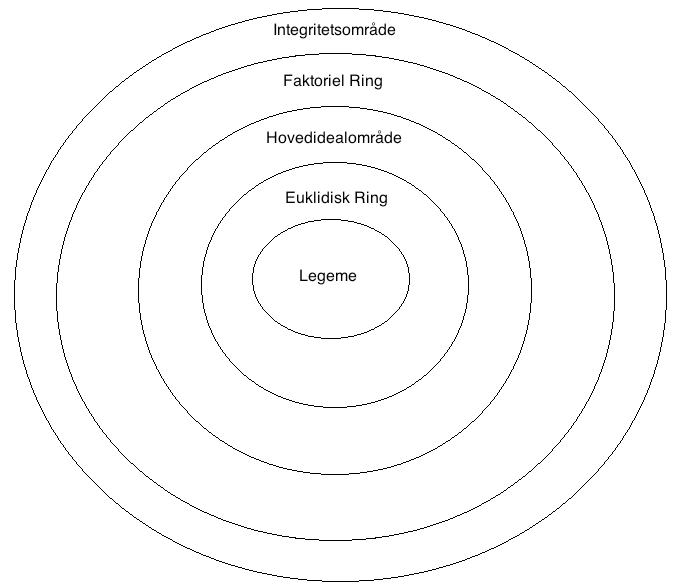
\includegraphics[width=0.8\textwidth]{img/ring_classes}











